\PassOptionsToPackage{unicode=true}{hyperref} % options for packages loaded elsewhere
\PassOptionsToPackage{hyphens}{url}
%
\documentclass[]{article}
\usepackage{lmodern}
\usepackage{amssymb,amsmath}
\usepackage{ifxetex,ifluatex}
\usepackage{fixltx2e} % provides \textsubscript
\ifnum 0\ifxetex 1\fi\ifluatex 1\fi=0 % if pdftex
  \usepackage[T1]{fontenc}
  \usepackage[utf8]{inputenc}
  \usepackage{textcomp} % provides euro and other symbols
\else % if luatex or xelatex
  \usepackage{unicode-math}
  \defaultfontfeatures{Ligatures=TeX,Scale=MatchLowercase}
\fi
% use upquote if available, for straight quotes in verbatim environments
\IfFileExists{upquote.sty}{\usepackage{upquote}}{}
% use microtype if available
\IfFileExists{microtype.sty}{%
\usepackage[]{microtype}
\UseMicrotypeSet[protrusion]{basicmath} % disable protrusion for tt fonts
}{}
\IfFileExists{parskip.sty}{%
\usepackage{parskip}
}{% else
\setlength{\parindent}{0pt}
\setlength{\parskip}{6pt plus 2pt minus 1pt}
}
\usepackage{hyperref}
\hypersetup{
            pdftitle={Data Replication Assignment},
            pdfauthor={Kelton Sheridan},
            pdfborder={0 0 0},
            breaklinks=true}
\urlstyle{same}  % don't use monospace font for urls
\usepackage[margin=1in]{geometry}
\usepackage{color}
\usepackage{fancyvrb}
\newcommand{\VerbBar}{|}
\newcommand{\VERB}{\Verb[commandchars=\\\{\}]}
\DefineVerbatimEnvironment{Highlighting}{Verbatim}{commandchars=\\\{\}}
% Add ',fontsize=\small' for more characters per line
\usepackage{framed}
\definecolor{shadecolor}{RGB}{248,248,248}
\newenvironment{Shaded}{\begin{snugshade}}{\end{snugshade}}
\newcommand{\AlertTok}[1]{\textcolor[rgb]{0.94,0.16,0.16}{#1}}
\newcommand{\AnnotationTok}[1]{\textcolor[rgb]{0.56,0.35,0.01}{\textbf{\textit{#1}}}}
\newcommand{\AttributeTok}[1]{\textcolor[rgb]{0.77,0.63,0.00}{#1}}
\newcommand{\BaseNTok}[1]{\textcolor[rgb]{0.00,0.00,0.81}{#1}}
\newcommand{\BuiltInTok}[1]{#1}
\newcommand{\CharTok}[1]{\textcolor[rgb]{0.31,0.60,0.02}{#1}}
\newcommand{\CommentTok}[1]{\textcolor[rgb]{0.56,0.35,0.01}{\textit{#1}}}
\newcommand{\CommentVarTok}[1]{\textcolor[rgb]{0.56,0.35,0.01}{\textbf{\textit{#1}}}}
\newcommand{\ConstantTok}[1]{\textcolor[rgb]{0.00,0.00,0.00}{#1}}
\newcommand{\ControlFlowTok}[1]{\textcolor[rgb]{0.13,0.29,0.53}{\textbf{#1}}}
\newcommand{\DataTypeTok}[1]{\textcolor[rgb]{0.13,0.29,0.53}{#1}}
\newcommand{\DecValTok}[1]{\textcolor[rgb]{0.00,0.00,0.81}{#1}}
\newcommand{\DocumentationTok}[1]{\textcolor[rgb]{0.56,0.35,0.01}{\textbf{\textit{#1}}}}
\newcommand{\ErrorTok}[1]{\textcolor[rgb]{0.64,0.00,0.00}{\textbf{#1}}}
\newcommand{\ExtensionTok}[1]{#1}
\newcommand{\FloatTok}[1]{\textcolor[rgb]{0.00,0.00,0.81}{#1}}
\newcommand{\FunctionTok}[1]{\textcolor[rgb]{0.00,0.00,0.00}{#1}}
\newcommand{\ImportTok}[1]{#1}
\newcommand{\InformationTok}[1]{\textcolor[rgb]{0.56,0.35,0.01}{\textbf{\textit{#1}}}}
\newcommand{\KeywordTok}[1]{\textcolor[rgb]{0.13,0.29,0.53}{\textbf{#1}}}
\newcommand{\NormalTok}[1]{#1}
\newcommand{\OperatorTok}[1]{\textcolor[rgb]{0.81,0.36,0.00}{\textbf{#1}}}
\newcommand{\OtherTok}[1]{\textcolor[rgb]{0.56,0.35,0.01}{#1}}
\newcommand{\PreprocessorTok}[1]{\textcolor[rgb]{0.56,0.35,0.01}{\textit{#1}}}
\newcommand{\RegionMarkerTok}[1]{#1}
\newcommand{\SpecialCharTok}[1]{\textcolor[rgb]{0.00,0.00,0.00}{#1}}
\newcommand{\SpecialStringTok}[1]{\textcolor[rgb]{0.31,0.60,0.02}{#1}}
\newcommand{\StringTok}[1]{\textcolor[rgb]{0.31,0.60,0.02}{#1}}
\newcommand{\VariableTok}[1]{\textcolor[rgb]{0.00,0.00,0.00}{#1}}
\newcommand{\VerbatimStringTok}[1]{\textcolor[rgb]{0.31,0.60,0.02}{#1}}
\newcommand{\WarningTok}[1]{\textcolor[rgb]{0.56,0.35,0.01}{\textbf{\textit{#1}}}}
\usepackage{graphicx,grffile}
\makeatletter
\def\maxwidth{\ifdim\Gin@nat@width>\linewidth\linewidth\else\Gin@nat@width\fi}
\def\maxheight{\ifdim\Gin@nat@height>\textheight\textheight\else\Gin@nat@height\fi}
\makeatother
% Scale images if necessary, so that they will not overflow the page
% margins by default, and it is still possible to overwrite the defaults
% using explicit options in \includegraphics[width, height, ...]{}
\setkeys{Gin}{width=\maxwidth,height=\maxheight,keepaspectratio}
\setlength{\emergencystretch}{3em}  % prevent overfull lines
\providecommand{\tightlist}{%
  \setlength{\itemsep}{0pt}\setlength{\parskip}{0pt}}
\setcounter{secnumdepth}{0}
% Redefines (sub)paragraphs to behave more like sections
\ifx\paragraph\undefined\else
\let\oldparagraph\paragraph
\renewcommand{\paragraph}[1]{\oldparagraph{#1}\mbox{}}
\fi
\ifx\subparagraph\undefined\else
\let\oldsubparagraph\subparagraph
\renewcommand{\subparagraph}[1]{\oldsubparagraph{#1}\mbox{}}
\fi

% set default figure placement to htbp
\makeatletter
\def\fps@figure{htbp}
\makeatother


\title{Data Replication Assignment}
\author{Kelton Sheridan}
\date{4/16/2020}

\begin{document}
\maketitle

\begin{verbatim}
The purpose of this paper was to determine where the ceramic sherds(pieces) originated in Peru by using Instrumental Neutron Activation Analysis, which will show the source of the clay used. 
\end{verbatim}

\hypertarget{neutron-activation-analysis-of-inca-and-colonial-ceramics}{%
\subsection{Neutron Activation Analysis of Inca and Colonial
Ceramics}\label{neutron-activation-analysis-of-inca-and-colonial-ceramics}}

\hypertarget{from-central-highland-ecuador}{%
\subsection{from Central Highland
Ecuador}\label{from-central-highland-ecuador}}

\begin{Shaded}
\begin{Highlighting}[]
\KeywordTok{library}\NormalTok{(readxl)}
\KeywordTok{library}\NormalTok{(ggplot2)}
\KeywordTok{library}\NormalTok{(tidyselect)}
\KeywordTok{library}\NormalTok{(dplyr)}
\CommentTok{#Reading in the data from table 1 in order to make table 2}
\NormalTok{f <-}\StringTok{ "data-reanalysis1.xlsx"}
\NormalTok{ceramic <-}\StringTok{ }\KeywordTok{read_excel}\NormalTok{(f, }\DataTypeTok{sheet =} \DecValTok{1}\NormalTok{, }\DataTypeTok{col_names =} \OtherTok{TRUE}\NormalTok{)}
\KeywordTok{head}\NormalTok{(ceramic)}
\end{Highlighting}
\end{Shaded}

\begin{verbatim}
## # A tibble: 6 x 31
##   Site   No.      Al    Ca    Dy    Mn    Ti     V     K    Na    As     U    La
##   <chr>  <chr> <dbl> <dbl> <dbl> <dbl> <dbl> <dbl> <dbl> <dbl> <dbl> <dbl> <dbl>
## 1 Spain  HUM ~   7.7   9.5   4     750  3030   126   1.2  0.95   4.3  1.67  31.6
## 2 Inca   QUI ~  11.3   1.3   1.1   271  3670   115   0.6  1.34   5.4  1.86  13.6
## 3 Panama LAM ~   8.8   4.6   1.2   878  3370   160   1.3  1.65   4.4  1.43  25.2
## 4 Panama LAM ~  10     1.9   4.2  1250  2570   111   1.3  1.32  10.7  1.58  28.4
## 5 Panama QUI ~   9.1   1.4   3.5   737  2810    85   1.6  1.49  16.4  2.86  25.5
## 6 Cuenca IGL ~   9.2   0.9   3.1   327  4030   106   0.8  0.99  17.6  1.81  17.7
## # ... with 18 more variables: Yb <dbl>, Sb <dbl>, Sm <dbl>, Ba <dbl>, Ce <dbl>,
## #   Co <dbl>, Cr <dbl>, Cs <dbl>, Eu <dbl>, Fe <dbl>, Tb <dbl>, Nd <dbl>,
## #   Ni <dbl>, Sc <dbl>, Sr <dbl>, Ta <dbl>, Th <dbl>, Hf <dbl>
\end{verbatim}

\begin{Shaded}
\begin{Highlighting}[]
\KeywordTok{summary}\NormalTok{(ceramic)}
\end{Highlighting}
\end{Shaded}

\begin{verbatim}
##      Site               No.                  Al              Ca       
##  Length:53          Length:53          Min.   : 7.40   Min.   :0.400  
##  Class :character   Class :character   1st Qu.: 9.20   1st Qu.:2.200  
##  Mode  :character   Mode  :character   Median : 9.50   Median :2.600  
##                                        Mean   : 9.56   Mean   :2.687  
##                                        3rd Qu.:10.00   3rd Qu.:3.400  
##                                        Max.   :12.00   Max.   :9.500  
##        Dy              Mn               Ti             V        
##  Min.   :1.000   Min.   : 271.0   Min.   :2380   Min.   : 64.0  
##  1st Qu.:1.500   1st Qu.: 653.0   1st Qu.:3020   1st Qu.:103.0  
##  Median :2.600   Median : 776.0   Median :3510   Median :127.0  
##  Mean   :2.487   Mean   : 797.3   Mean   :3552   Mean   :128.5  
##  3rd Qu.:3.100   3rd Qu.: 934.0   3rd Qu.:4000   3rd Qu.:157.0  
##  Max.   :4.700   Max.   :1250.0   Max.   :5420   Max.   :204.0  
##        K                Na              As               U        
##  Min.   :0.3000   Min.   :0.420   Min.   : 1.300   Min.   :0.430  
##  1st Qu.:0.6000   1st Qu.:1.580   1st Qu.: 2.000   1st Qu.:0.850  
##  Median :0.7000   Median :1.850   Median : 3.500   Median :1.300  
##  Mean   :0.7283   Mean   :1.716   Mean   : 5.908   Mean   :1.325  
##  3rd Qu.:0.8000   3rd Qu.:2.010   3rd Qu.: 6.300   3rd Qu.:1.690  
##  Max.   :1.6000   Max.   :2.310   Max.   :22.300   Max.   :2.890  
##        La              Yb              Sb               Sm       
##  Min.   :13.60   Min.   :0.780   Min.   :0.1100   Min.   :2.610  
##  1st Qu.:18.00   1st Qu.:1.080   1st Qu.:0.3100   1st Qu.:3.740  
##  Median :22.60   Median :1.260   Median :0.4500   Median :4.220  
##  Mean   :23.43   Mean   :1.447   Mean   :0.9658   Mean   :4.356  
##  3rd Qu.:26.50   3rd Qu.:1.610   3rd Qu.:1.4600   3rd Qu.:4.900  
##  Max.   :37.40   Max.   :3.090   Max.   :4.5900   Max.   :6.610  
##        Ba               Ce              Co              Cr        
##  Min.   : 410.0   Min.   :24.40   Min.   : 4.70   Min.   : 18.00  
##  1st Qu.: 660.0   1st Qu.:37.10   1st Qu.:10.70   1st Qu.: 34.00  
##  Median : 721.0   Median :44.60   Median :15.20   Median : 41.00  
##  Mean   : 743.7   Mean   :46.84   Mean   :15.34   Mean   : 57.49  
##  3rd Qu.: 828.0   3rd Qu.:55.10   3rd Qu.:19.50   3rd Qu.: 89.00  
##  Max.   :1360.0   Max.   :77.10   Max.   :27.30   Max.   :115.00  
##        Cs               Eu              Fe             Tb        
##  Min.   : 1.070   Min.   :0.700   Min.   :2.96   Min.   :0.2100  
##  1st Qu.: 2.420   1st Qu.:1.000   1st Qu.:3.85   1st Qu.:0.4800  
##  Median : 2.800   Median :1.200   Median :4.33   Median :0.5500  
##  Mean   : 4.381   Mean   :1.147   Mean   :4.28   Mean   :0.5857  
##  3rd Qu.: 4.160   3rd Qu.:1.300   3rd Qu.:4.75   3rd Qu.:0.6900  
##  Max.   :18.900   Max.   :1.600   Max.   :6.13   Max.   :1.0200  
##        Nd              Ni              Sc              Sr       
##  Min.   : 5.00   Min.   :38.00   Min.   : 8.74   Min.   : 64.0  
##  1st Qu.:16.00   1st Qu.:43.00   1st Qu.:10.30   1st Qu.:270.0  
##  Median :22.00   Median :46.00   Median :13.30   Median :326.0  
##  Mean   :21.49   Mean   :47.32   Mean   :13.03   Mean   :325.7  
##  3rd Qu.:27.00   3rd Qu.:50.00   3rd Qu.:15.10   3rd Qu.:408.0  
##  Max.   :37.00   Max.   :60.00   Max.   :22.80   Max.   :731.0  
##        Ta               Th               Hf       
##  Min.   :0.2300   Min.   : 4.100   Min.   :3.500  
##  1st Qu.:0.4900   1st Qu.: 5.700   1st Qu.:4.300  
##  Median :0.6300   Median : 7.300   Median :5.000  
##  Mean   :0.6587   Mean   : 7.508   Mean   :5.183  
##  3rd Qu.:0.8600   3rd Qu.: 8.900   3rd Qu.:5.500  
##  Max.   :1.2700   Max.   :14.400   Max.   :9.000
\end{verbatim}

\begin{Shaded}
\begin{Highlighting}[]
\CommentTok{#For all of the cells that has a less than symbol, I  made them equal to instead,}
\CommentTok{#which may end up changing the results a tiny bit.}
\CommentTok{#In order to create Table 2 from the article, I used group_by and summarize to find}
\CommentTok{#the means.}
\NormalTok{s <-}\StringTok{ }\KeywordTok{group_by}\NormalTok{(ceramic, Site) }\OperatorTok
\StringTok{  }\KeywordTok{summarize}\NormalTok{(}
  \DataTypeTok{meanAL =} \KeywordTok{mean}\NormalTok{(Al),}
  \DataTypeTok{meanCA =} \KeywordTok{mean}\NormalTok{(Ca),}
  \DataTypeTok{meanDy =} \KeywordTok{mean}\NormalTok{(Dy),}
  \DataTypeTok{meanMn =} \KeywordTok{mean}\NormalTok{(Mn),}
  \DataTypeTok{meanTi =} \KeywordTok{mean}\NormalTok{(Ti),}
  \DataTypeTok{meanV =} \KeywordTok{mean}\NormalTok{(V),}
  \DataTypeTok{meanK =} \KeywordTok{mean}\NormalTok{(K),}
  \DataTypeTok{meanNa =} \KeywordTok{mean}\NormalTok{(Na),}
  \DataTypeTok{meanAs =} \KeywordTok{mean}\NormalTok{(As), }
  \DataTypeTok{meanU =} \KeywordTok{mean}\NormalTok{(U),}
  \DataTypeTok{meanLa =} \KeywordTok{mean}\NormalTok{(La),}
  \DataTypeTok{meanYb =} \KeywordTok{mean}\NormalTok{(Yb),}
  \DataTypeTok{meanSb =} \KeywordTok{mean}\NormalTok{(Sb), }
  \DataTypeTok{meanSm =} \KeywordTok{mean}\NormalTok{(Sm), }
  \DataTypeTok{meanBa =} \KeywordTok{mean}\NormalTok{(Ba),}
  \DataTypeTok{meanCe =} \KeywordTok{mean}\NormalTok{(Ce),}
  \DataTypeTok{meanCo =} \KeywordTok{mean}\NormalTok{(Co),}
  \DataTypeTok{meanCr =} \KeywordTok{mean}\NormalTok{(Cr),}
  \DataTypeTok{meanCs =} \KeywordTok{mean}\NormalTok{(Cs),}
  \DataTypeTok{meanEu =} \KeywordTok{mean}\NormalTok{(Eu),}
  \DataTypeTok{meanFe =} \KeywordTok{mean}\NormalTok{(Fe),}
  \DataTypeTok{meanTb =} \KeywordTok{mean}\NormalTok{(Tb),}
  \DataTypeTok{meanNd =} \KeywordTok{mean}\NormalTok{(Nd),}
  \DataTypeTok{meanNi =} \KeywordTok{mean}\NormalTok{(Ni),}
  \DataTypeTok{meanSc =} \KeywordTok{mean}\NormalTok{(Sc),}
  \DataTypeTok{meanSr =} \KeywordTok{mean}\NormalTok{(Sr),}
  \DataTypeTok{meanTa =} \KeywordTok{mean}\NormalTok{(Ta),}
  \DataTypeTok{meanTh =} \KeywordTok{mean}\NormalTok{(Th),}
  \DataTypeTok{meanHf =} \KeywordTok{mean}\NormalTok{(Hf)}
\NormalTok{  )}
\NormalTok{  s}
\end{Highlighting}
\end{Shaded}

\begin{verbatim}
## # A tibble: 6 x 30
##   Site  meanAL meanCA meanDy meanMn meanTi meanV meanK meanNa meanAs meanU
##   <chr>  <dbl>  <dbl>  <dbl>  <dbl>  <dbl> <dbl> <dbl>  <dbl>  <dbl> <dbl>
## 1 Cuen~   8.17  0.771   3.13   672.  4389.  101. 0.743  0.791  17.0  2.16 
## 2 Inca   11.3   1.3     1.1    271   3670   115  0.6    1.34    5.4  1.86 
## 3 Pana~   9.3   2.63    2.97   955   2917.  119. 1.4    1.49   10.5  1.96 
## 4 Quito   9.71  2.50    2.19   732.  3091.  110. 0.724  1.97    5.39 1.28 
## 5 Riob~   9.93  3.28    2.50   915.  3860.  160. 0.61   1.87    1.98 0.937
## 6 Spain   7.7   9.5     4      750   3030   126  1.2    0.95    4.3  1.67 
## # ... with 19 more variables: meanLa <dbl>, meanYb <dbl>, meanSb <dbl>,
## #   meanSm <dbl>, meanBa <dbl>, meanCe <dbl>, meanCo <dbl>, meanCr <dbl>,
## #   meanCs <dbl>, meanEu <dbl>, meanFe <dbl>, meanTb <dbl>, meanNd <dbl>,
## #   meanNi <dbl>, meanSc <dbl>, meanSr <dbl>, meanTa <dbl>, meanTh <dbl>,
## #   meanHf <dbl>
\end{verbatim}

\hypertarget{figure-4}{%
\subsection{Figure 4}\label{figure-4}}

\begin{verbatim}
##  [1] "Site" "No."  "Al"   "Ca"   "Dy"   "Mn"   "Ti"   "V"    "K"    "Na"  
## [11] "As"   "U"    "La"   "Yb"   "Sb"   "Sm"   "Ba"   "Ce"   "Co"   "Cr"  
## [21] "Cs"   "Eu"   "Fe"   "Tb"   "Nd"   "Ni"   "Sc"   "Sr"   "Ta"   "Th"  
## [31] "Hf"
\end{verbatim}

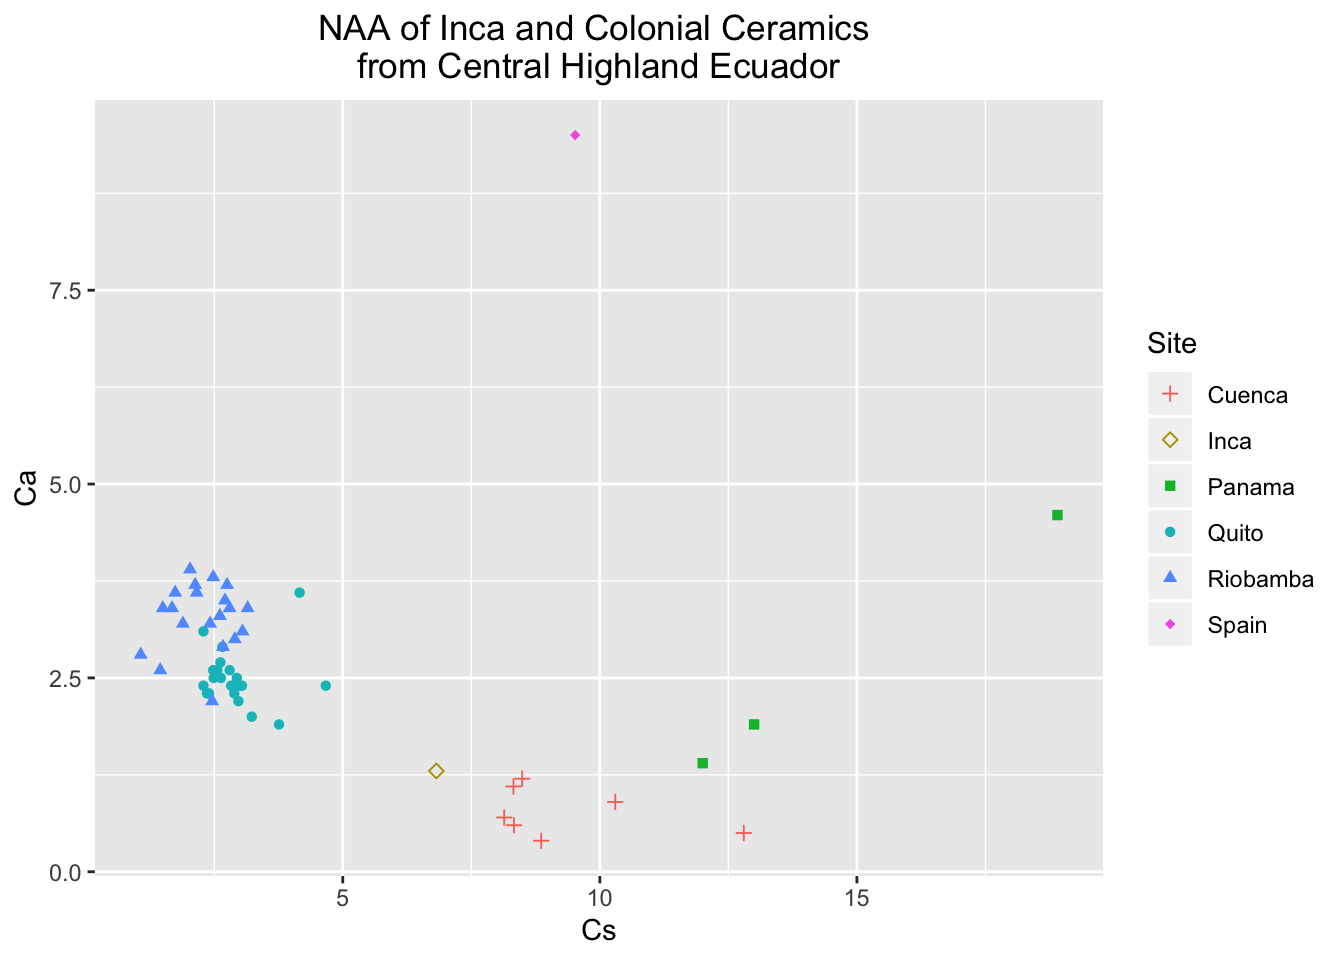
\includegraphics{RMD-Sheridan_Reanalysis_files/figure-latex/pressure-1.pdf}

\hypertarget{figure-6}{%
\subsection{Figure 6}\label{figure-6}}

\begin{verbatim}
##  [1] "Site" "No."  "Al"   "Ca"   "Dy"   "Mn"   "Ti"   "V"    "K"    "Na"  
## [11] "As"   "U"    "La"   "Yb"   "Sb"   "Sm"   "Ba"   "Ce"   "Co"   "Cr"  
## [21] "Cs"   "Eu"   "Fe"   "Tb"   "Nd"   "Ni"   "Sc"   "Sr"   "Ta"   "Th"  
## [31] "Hf"
\end{verbatim}

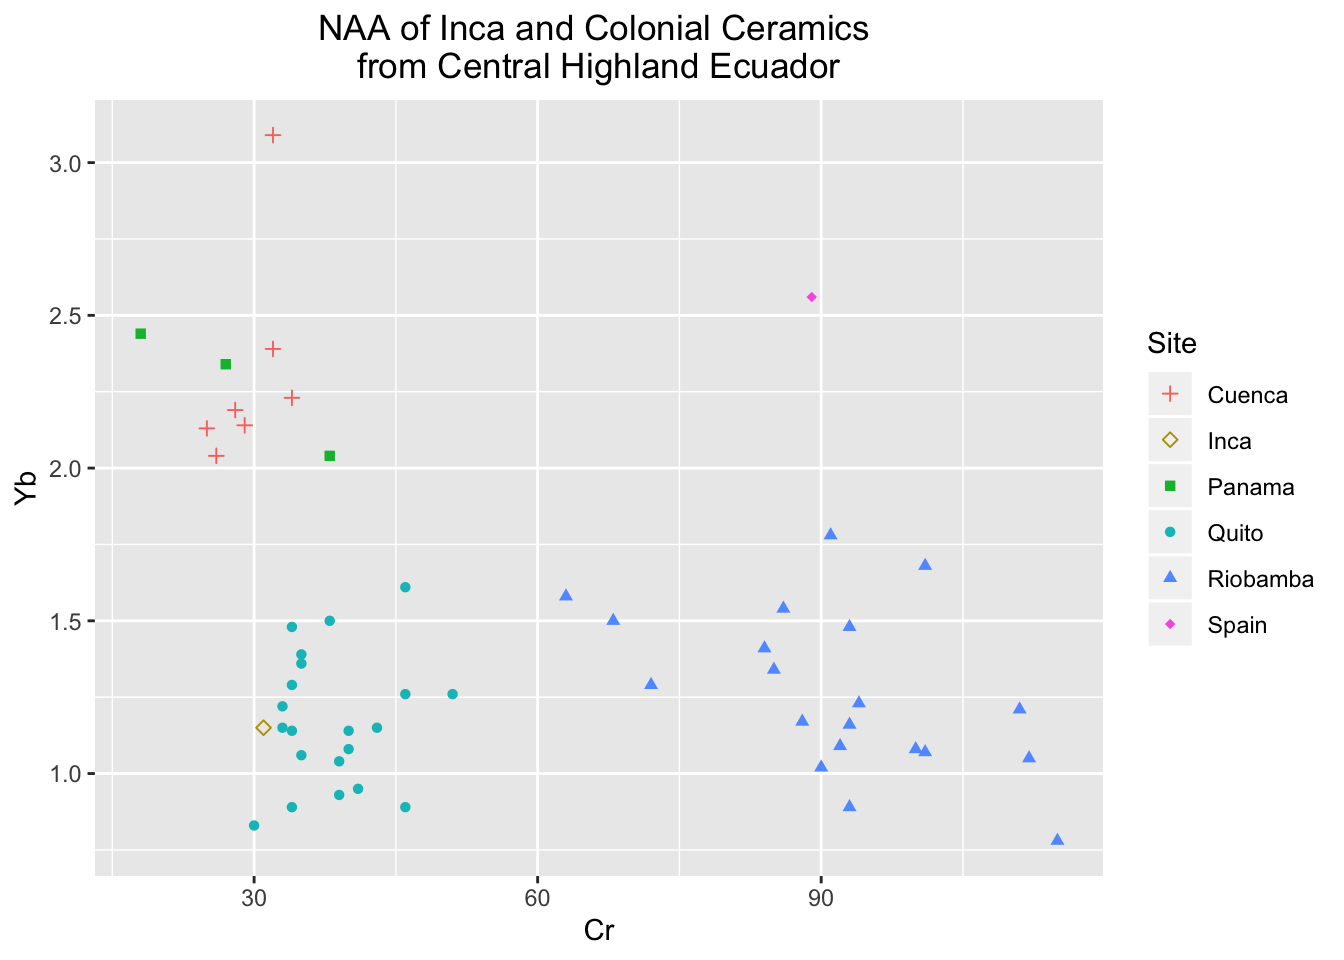
\includegraphics{RMD-Sheridan_Reanalysis_files/figure-latex/pressures-1.pdf}

Note that the \texttt{echo\ =\ FALSE} parameter was added to the code
chunk to prevent printing of the R code that generated the plot.

\end{document}
